\documentclass[a4paper,11pt]{article}
\usepackage[utf8]{inputenc}
\usepackage[T1]{fontenc}
\usepackage[english]{babel}
\usepackage{lmodern}\usepackage{microtype}
\usepackage{amsmath,amssymb,bm,mathtools}
\usepackage{geometry}
\geometry{a4paper,left=2.3cm,right=2.3cm,top=2.0cm,bottom=2.0cm}
\usepackage{booktabs,array}
\usepackage{xcolor}\definecolor{bokug}{RGB}{0,135,60}
\usepackage{tikz}
\usetikzlibrary{patterns,arrows.meta,calc,decorations.pathmorphing}
\usepackage{fancyhdr}\pagestyle{fancy}
\renewcommand{\headrulewidth}{0.4pt}
\usepackage{enumitem}\setlength{\parindent}{0pt}\setlength{\parskip}{4pt}

\begin{document}
\fancyhead[L]{\small VU Mechanik – LAWI 100515 (PI)}
\fancyhead[R]{\small SS 2026}
\fancyfoot[C]{\thepage}
\begin{center}{\large\bfseries\color{bokug}University of Natural Resources and Life Sciences, Vienna (BOKU)}\\[2pt]{\large\bfseries VU Mechanik – LAWI 100515 (PI)}\\[4pt]Exam \textbf{Group A} \hfill Date: 26.06.2026\\[2pt]\rule{\linewidth}{0.4pt}\end{center}

\begin{center}\textbf{\large Model solution}\end{center}
\begin{center}
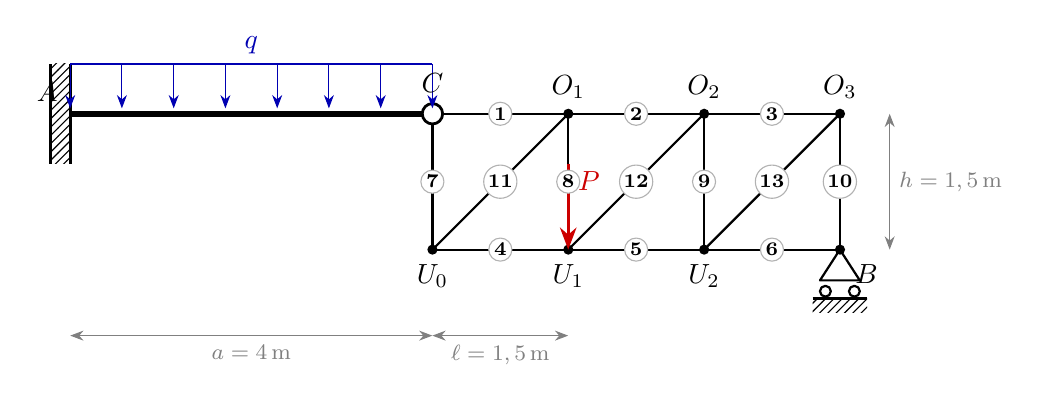
\begin{tikzpicture}[scale=1.15, >=Stealth, line join=round]
  \coordinate (A) at (0.000,0.000);
  \coordinate (C) at (4.000,0.000);
  \coordinate (O1) at (5.500,0.000);
  \coordinate (O2) at (7.000,0.000);
  \coordinate (O3) at (8.500,0.000);
  \coordinate (U0) at (4.000,-1.500);
  \coordinate (U1) at (5.500,-1.500);
  \coordinate (U2) at (7.000,-1.500);
  \coordinate (U3) at (8.500,-1.500);
  \draw[thick] (C) -- (O1);
  \draw[thick] (O1) -- (O2);
  \draw[thick] (O2) -- (O3);
  \draw[thick] (U0) -- (U1);
  \draw[thick] (U1) -- (U2);
  \draw[thick] (U2) -- (U3);
  \draw[thick] (C) -- (U0);
  \draw[thick] (O1) -- (U1);
  \draw[thick] (O2) -- (U2);
  \draw[thick] (O3) -- (U3);
  \draw[thick] (U0) -- (O1);
  \draw[thick] (U1) -- (O2);
  \draw[thick] (U2) -- (O3);
  \draw[line width=2.2pt] (A) -- (C);
  \fill (C) circle (1.6pt);
  \fill (O1) circle (1.6pt);
  \fill (O2) circle (1.6pt);
  \fill (O3) circle (1.6pt);
  \fill (U0) circle (1.6pt);
  \fill (U1) circle (1.6pt);
  \fill (U2) circle (1.6pt);
  \fill (U3) circle (1.6pt);
  \draw[fill=white,line width=1pt] (C) circle (3.2pt);
  \draw[line width=1.1pt] (0.000,-0.550) -- (0.000,0.550);
  \fill[pattern=north east lines] (-0.220,-0.550) rectangle (0.000,0.550);
  \draw[line width=1.1pt] (-0.220,-0.550) -- (-0.220,0.550);
  \draw[thick] (8.500,-1.500) -- (8.280,-1.840) -- (8.720,-1.840) -- cycle;
  \draw[thick] (8.340,-1.960) circle (0.06) (8.660,-1.960) circle (0.06);
  \draw[line width=1.1pt] (8.200,-2.040) -- (8.800,-2.040);
  \fill[pattern=north east lines] (8.200,-2.200) rectangle (8.800,-2.040);
  \draw[blue!70!black,thick] (0.000,0.550) -- (4.000,0.550);
  \draw[->,blue!70!black] (0.000,0.550) -- (0.000,0.06);
  \draw[->,blue!70!black] (0.571,0.550) -- (0.571,0.06);
  \draw[->,blue!70!black] (1.143,0.550) -- (1.143,0.06);
  \draw[->,blue!70!black] (1.714,0.550) -- (1.714,0.06);
  \draw[->,blue!70!black] (2.286,0.550) -- (2.286,0.06);
  \draw[->,blue!70!black] (2.857,0.550) -- (2.857,0.06);
  \draw[->,blue!70!black] (3.429,0.550) -- (3.429,0.06);
  \draw[->,blue!70!black] (4.000,0.550) -- (4.000,0.06);
  \node[blue!70!black,above] at (2.000,0.550) {$q$};
  \draw[->,red!80!black,line width=1.1pt] (5.500,-0.550) -- (5.500,-1.500);
  \node[red!80!black,above right] at (5.500,-0.950) {$P$};
  \node[circle,fill=white,draw=gray!60,inner sep=0.7pt,font=\scriptsize] at (4.750,0.000) {\textbf{1}};
  \node[circle,fill=white,draw=gray!60,inner sep=0.7pt,font=\scriptsize] at (6.250,0.000) {\textbf{2}};
  \node[circle,fill=white,draw=gray!60,inner sep=0.7pt,font=\scriptsize] at (7.750,0.000) {\textbf{3}};
  \node[circle,fill=white,draw=gray!60,inner sep=0.7pt,font=\scriptsize] at (4.750,-1.500) {\textbf{4}};
  \node[circle,fill=white,draw=gray!60,inner sep=0.7pt,font=\scriptsize] at (6.250,-1.500) {\textbf{5}};
  \node[circle,fill=white,draw=gray!60,inner sep=0.7pt,font=\scriptsize] at (7.750,-1.500) {\textbf{6}};
  \node[circle,fill=white,draw=gray!60,inner sep=0.7pt,font=\scriptsize] at (4.000,-0.750) {\textbf{7}};
  \node[circle,fill=white,draw=gray!60,inner sep=0.7pt,font=\scriptsize] at (5.500,-0.750) {\textbf{8}};
  \node[circle,fill=white,draw=gray!60,inner sep=0.7pt,font=\scriptsize] at (7.000,-0.750) {\textbf{9}};
  \node[circle,fill=white,draw=gray!60,inner sep=0.7pt,font=\scriptsize] at (8.500,-0.750) {\textbf{10}};
  \node[circle,fill=white,draw=gray!60,inner sep=0.7pt,font=\scriptsize] at (4.750,-0.750) {\textbf{11}};
  \node[circle,fill=white,draw=gray!60,inner sep=0.7pt,font=\scriptsize] at (6.250,-0.750) {\textbf{12}};
  \node[circle,fill=white,draw=gray!60,inner sep=0.7pt,font=\scriptsize] at (7.750,-0.750) {\textbf{13}};
  \node[above left=1pt] at (A) {$A$};
  \node[above=4pt] at (C) {$C$};
  \node[above=2pt] at (O1) {$O_{1}$};
  \node[above=2pt] at (O2) {$O_{2}$};
  \node[above=2pt] at (O3) {$O_{3}$};
  \node[below=2pt] at (U0) {$U_{0}$};
  \node[below=2pt] at (U1) {$U_{1}$};
  \node[below=2pt] at (U2) {$U_{2}$};
  \node[below right=2pt] at (U3) {$B$};
  \draw[<->,gray] (0.000,-2.450) -- (4.000,-2.450) node[midway,below,font=\footnotesize]{$a=4$\,m};
  \draw[<->,gray] (4.000,-2.450) -- (5.500,-2.450) node[midway,below,font=\footnotesize]{$\ell=1,5$\,m};
  \draw[<->,gray] (9.050,0) -- (9.050,-1.500) node[midway,right,font=\footnotesize]{$h=1,5$\,m};
\end{tikzpicture}
\end{center}
\par\medskip\textbf{1.\ Static determinacy}\\[-2pt]
Counting criterion $n = r - (3 + v)$ with $r$ support reactions and $v$ hinge conditions:
\[ n = r - (3+v) = 4 - (3+1) = 0 \quad\Rightarrow\quad \text{the system is statically determinate.} \]
\par\medskip\textbf{2.\ Support reactions and hinge force}\\[-2pt]
$A_x = 0$\,kN,\quad $A_y = 30.67$\,kN,\quad $M_A = 74.67$\,kNm,\quad $B_y = 3.33$\,kN\\[2pt]$C_x = 0$\,kN,\quad $C_y = -6.67$\,kN\par
\par\medskip\textbf{3.\ Truss member forces}\par
\begin{center}\renewcommand{\arraystretch}{1.15}
\begin{tabular}{c r l}
\toprule
Member & Member force $S$ [kN] & Type \\
\midrule
  1 (C\,--\,O1) & 0 & zero-force \\
  2 (O1\,--\,O2) & -6.67 & compression \\
  3 (O2\,--\,O3) & -3.33 & compression \\
  4 (U0\,--\,U1) & 6.67 & tension \\
  5 (U1\,--\,U2) & 3.33 & tension \\
  6 (U2\,--\,U3) & 0 & zero-force \\
  7 (C\,--\,U0) & 6.67 & tension \\
  8 (O1\,--\,U1) & 6.67 & tension \\
  9 (O2\,--\,U2) & -3.33 & compression \\
  10 (O3\,--\,U3) & -3.33 & compression \\
  11 (U0\,--\,O1) & -9.43 & compression \\
  12 (U1\,--\,O2) & 4.71 & tension \\
  13 (U2\,--\,O3) & 4.71 & tension \\
\bottomrule
\end{tabular}\end{center}
\begin{center}
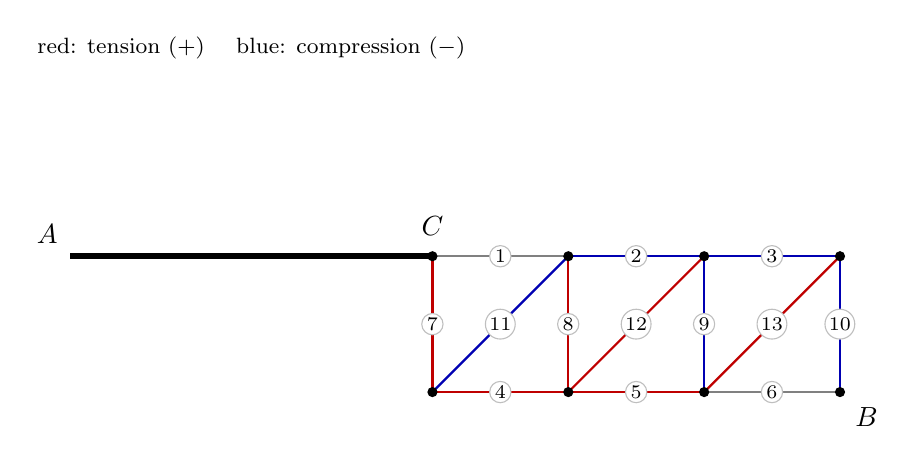
\begin{tikzpicture}[scale=1.15, >=Stealth, line join=round]
  \coordinate (A) at (0.000,0.000);
  \coordinate (C) at (4.000,0.000);
  \coordinate (O1) at (5.500,0.000);
  \coordinate (O2) at (7.000,0.000);
  \coordinate (O3) at (8.500,0.000);
  \coordinate (U0) at (4.000,-1.500);
  \coordinate (U1) at (5.500,-1.500);
  \coordinate (U2) at (7.000,-1.500);
  \coordinate (U3) at (8.500,-1.500);
  \draw[thick,gray] (C) -- (O1);
  \draw[thick,blue!70!black] (O1) -- (O2);
  \draw[thick,blue!70!black] (O2) -- (O3);
  \draw[thick,red!75!black] (U0) -- (U1);
  \draw[thick,red!75!black] (U1) -- (U2);
  \draw[thick,gray] (U2) -- (U3);
  \draw[thick,red!75!black] (C) -- (U0);
  \draw[thick,red!75!black] (O1) -- (U1);
  \draw[thick,blue!70!black] (O2) -- (U2);
  \draw[thick,blue!70!black] (O3) -- (U3);
  \draw[thick,blue!70!black] (U0) -- (O1);
  \draw[thick,red!75!black] (U1) -- (O2);
  \draw[thick,red!75!black] (U2) -- (O3);
  \draw[line width=2.2pt] (A) -- (C);
  \fill (C) circle (1.6pt);
  \fill (O1) circle (1.6pt);
  \fill (O2) circle (1.6pt);
  \fill (O3) circle (1.6pt);
  \fill (U0) circle (1.6pt);
  \fill (U1) circle (1.6pt);
  \fill (U2) circle (1.6pt);
  \fill (U3) circle (1.6pt);
  \node[circle,fill=white,draw=gray!50,inner sep=0.6pt,font=\scriptsize] at (4.750,0.000) {1};
  \node[circle,fill=white,draw=gray!50,inner sep=0.6pt,font=\scriptsize] at (6.250,0.000) {2};
  \node[circle,fill=white,draw=gray!50,inner sep=0.6pt,font=\scriptsize] at (7.750,0.000) {3};
  \node[circle,fill=white,draw=gray!50,inner sep=0.6pt,font=\scriptsize] at (4.750,-1.500) {4};
  \node[circle,fill=white,draw=gray!50,inner sep=0.6pt,font=\scriptsize] at (6.250,-1.500) {5};
  \node[circle,fill=white,draw=gray!50,inner sep=0.6pt,font=\scriptsize] at (7.750,-1.500) {6};
  \node[circle,fill=white,draw=gray!50,inner sep=0.6pt,font=\scriptsize] at (4.000,-0.750) {7};
  \node[circle,fill=white,draw=gray!50,inner sep=0.6pt,font=\scriptsize] at (5.500,-0.750) {8};
  \node[circle,fill=white,draw=gray!50,inner sep=0.6pt,font=\scriptsize] at (7.000,-0.750) {9};
  \node[circle,fill=white,draw=gray!50,inner sep=0.6pt,font=\scriptsize] at (8.500,-0.750) {10};
  \node[circle,fill=white,draw=gray!50,inner sep=0.6pt,font=\scriptsize] at (4.750,-0.750) {11};
  \node[circle,fill=white,draw=gray!50,inner sep=0.6pt,font=\scriptsize] at (6.250,-0.750) {12};
  \node[circle,fill=white,draw=gray!50,inner sep=0.6pt,font=\scriptsize] at (7.750,-0.750) {13};
  \node[above left=1pt] at (A) {$A$};
  \node[above=4pt] at (C) {$C$};
  \node[below right=2pt] at (U3) {$B$};
  \node[font=\footnotesize,align=center] at (2.00,2.30) {red: tension $(+)$ \quad blue: compression $(-)$};
\end{tikzpicture}
\end{center}
\par\medskip\textbf{4.\ Section-force diagrams of the bending beam $A$--$C$}\par
\begin{center}
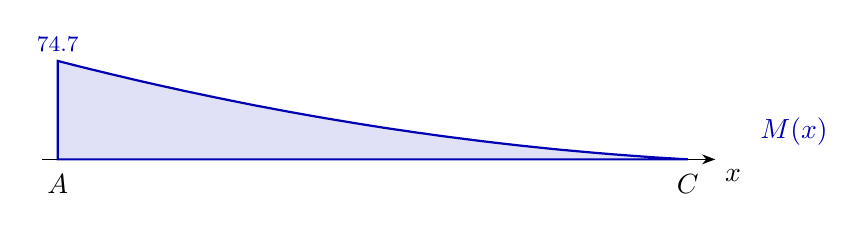
\begin{tikzpicture}[>=Stealth]
  \draw[->] (-0.2,0) -- (8.35,0) node[below right]{$x$};
  \node[below=2pt] at (0,0) {$A$};
  \node[below=2pt] at (8.00,0) {$C$};
  \filldraw[fill=blue!70!black!12,draw=blue!70!black,thick] (0,0) -- plot coordinates {(0.000,1.250) (0.133,1.216) (0.267,1.182) (0.400,1.149) (0.533,1.117) (0.667,1.084) (0.800,1.053) (0.933,1.021) (1.067,0.990) (1.200,0.960) (1.333,0.930) (1.467,0.901) (1.600,0.871) (1.733,0.843) (1.867,0.815) (2.000,0.787) (2.133,0.760) (2.267,0.733) (2.400,0.706) (2.533,0.680) (2.667,0.655) (2.800,0.630) (2.933,0.605) (3.067,0.581) (3.200,0.557) (3.333,0.534) (3.467,0.511) (3.600,0.489) (3.733,0.467) (3.867,0.445) (4.000,0.424) (4.133,0.403) (4.267,0.383) (4.400,0.364) (4.533,0.344) (4.667,0.326) (4.800,0.307) (4.933,0.289) (5.067,0.272) (5.200,0.255) (5.333,0.238) (5.467,0.222) (5.600,0.206) (5.733,0.191) (5.867,0.176) (6.000,0.162) (6.133,0.148) (6.267,0.134) (6.400,0.121) (6.533,0.109) (6.667,0.097) (6.800,0.085) (6.933,0.074) (7.067,0.063) (7.200,0.053) (7.333,0.043) (7.467,0.033) (7.600,0.024) (7.733,0.016) (7.867,0.008) (8.000,-0.000)} -- (8.000,0) -- cycle;
  \node[above,blue!70!black,font=\footnotesize] at (0.000,1.250) {74.7};
  \node[blue!70!black,right] at (8.80,0.35) {$M(x)$};
\end{tikzpicture}
\\[6pt]
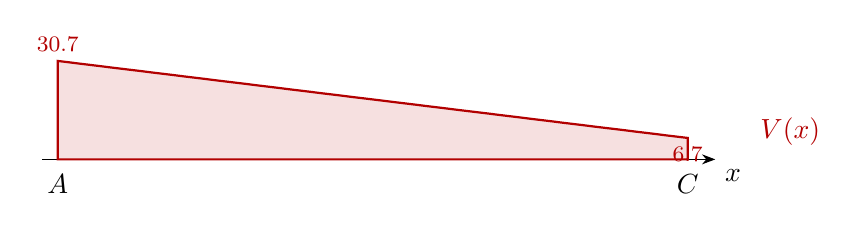
\begin{tikzpicture}[>=Stealth]
  \draw[->] (-0.2,0) -- (8.35,0) node[below right]{$x$};
  \node[below=2pt] at (0,0) {$A$};
  \node[below=2pt] at (8.00,0) {$C$};
  \filldraw[fill=red!70!black!12,draw=red!70!black,thick] (0,0) -- plot coordinates {(0.000,1.250) (0.133,1.234) (0.267,1.217) (0.400,1.201) (0.533,1.185) (0.667,1.168) (0.800,1.152) (0.933,1.136) (1.067,1.120) (1.200,1.103) (1.333,1.087) (1.467,1.071) (1.600,1.054) (1.733,1.038) (1.867,1.022) (2.000,1.005) (2.133,0.989) (2.267,0.973) (2.400,0.957) (2.533,0.940) (2.667,0.924) (2.800,0.908) (2.933,0.891) (3.067,0.875) (3.200,0.859) (3.333,0.842) (3.467,0.826) (3.600,0.810) (3.733,0.793) (3.867,0.777) (4.000,0.761) (4.133,0.745) (4.267,0.728) (4.400,0.712) (4.533,0.696) (4.667,0.679) (4.800,0.663) (4.933,0.647) (5.067,0.630) (5.200,0.614) (5.333,0.598) (5.467,0.582) (5.600,0.565) (5.733,0.549) (5.867,0.533) (6.000,0.516) (6.133,0.500) (6.267,0.484) (6.400,0.467) (6.533,0.451) (6.667,0.435) (6.800,0.418) (6.933,0.402) (7.067,0.386) (7.200,0.370) (7.333,0.353) (7.467,0.337) (7.600,0.321) (7.733,0.304) (7.867,0.288) (8.000,0.272)} -- (8.000,0) -- cycle;
  \node[above,red!70!black,font=\footnotesize] at (0.000,1.250) {30.7};
  \node[below,red!70!black,font=\footnotesize] at (8.000,0.272) {6.7};
  \node[red!70!black,right] at (8.80,0.35) {$V(x)$};
\end{tikzpicture}
\\[6pt]
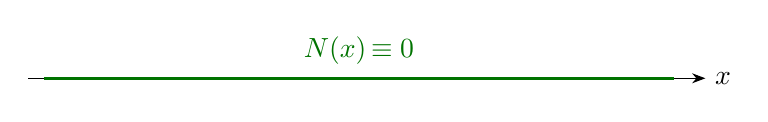
\begin{tikzpicture}[>=Stealth]
  \draw[->] (-0.2,0) -- (8.40,0) node[right]{$x$};
  \draw[green!45!black,very thick] (0,0) -- (8,0);
  \node[green!45!black] at (4,0.35) {$N(x)$\,$\equiv 0$};
\end{tikzpicture}
\end{center}
\end{document}